\textbf{Problem 16.} \\
\hrule 

Some parts of California are particularly earthquake prone. Suppose that in one metropolitan area, 25\% of all homeowners are insured against earthquake damage. Four homeowners are to be selected at random; let X denote the number among the four who have earthquake insurance.

\textbf{a. Find the probability distribution of X.} \textit{Hint:} Let S denote a homeowner who has insurance and F one who does not. Then one possible outcome is SFSS, with probability (.25)(.75)(.25)(.25) and associated X value 3. There are 15 other outcomes. 

\begin{table}[h]
\begin{tabular}{ll}
\hline
x & P[X = x] \\ \hline
0 & $\left( \frac{3}{4} \right)^4 \approx .316$ \\[1.5mm]
1 & $\binom{4}{1} \cdot \frac{1}{4} \cdot \left( \frac{3}{4} \right)^3 \approx .422 $ \\[1.5mm]
2 & $\binom{4}{2} \cdot \left( \frac{1}{4} \right)^2 \cdot \left( \frac{3}{4} \right)^2 \approx .211$  \\[1.5mm]
3 & $\binom{4}{3} \cdot \left( \frac{1}{4} \right)^3 \cdot \left( \frac{3}{4} \right) \approx .047$  \\[1.5mm]
4 & $\left( \frac{1}{4} \right)^4 \approx .0039$ \\[.5mm] \hline
& $\sum_{x}P[X=x]=.999$ \\
\multicolumn{1}{}{} & 
\end{tabular}
\end{table}

\textbf{b. Draw the corresponding probability histogram.}

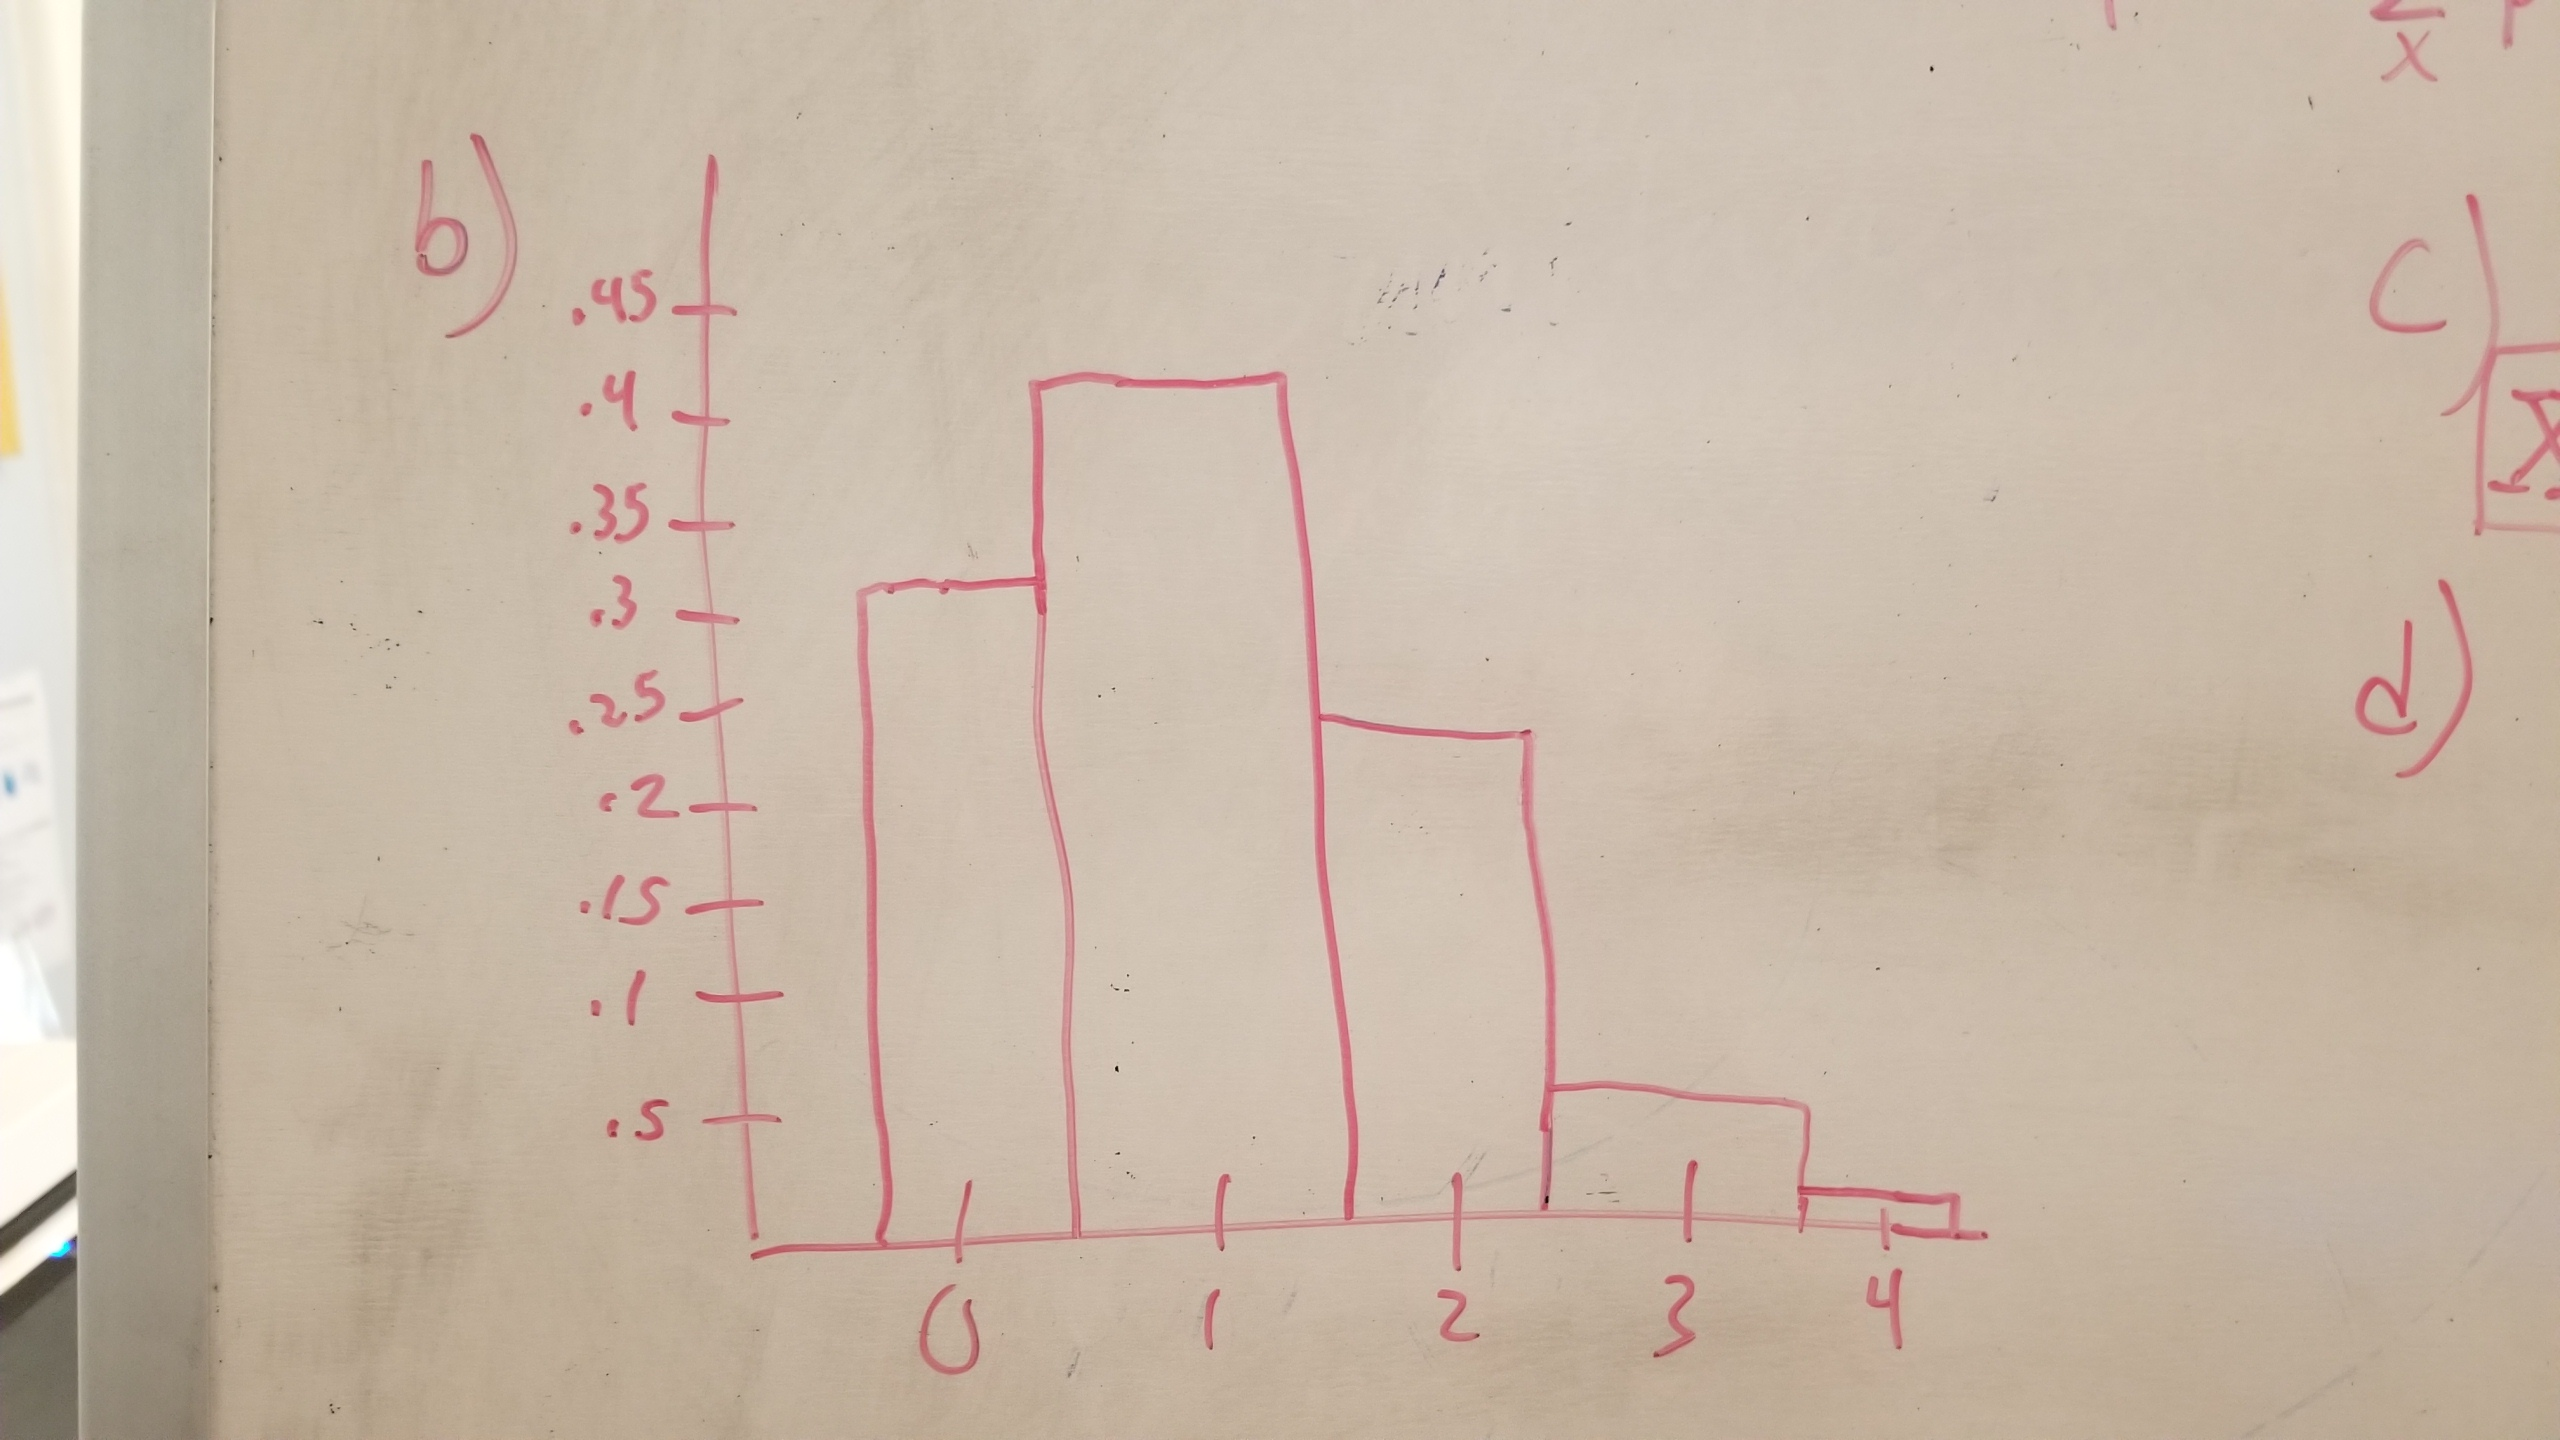
\includegraphics[scale=0.125]{images/whw4/3.2.16.jpg}

\textbf{c. What is the most likely value for X?}

\[\boxed{X = 1}\]

\textbf{d. What is the probability that at least two of the four selected have earthquake insurance?}

\[P[X \geq 2] \approx \boxed{.2619}\]